\documentclass[11pt,a4paper]{article}
\usepackage{fontspec}
\setmainfont{Latin Modern Roman}\setsansfont{Latin Modern Sans}\setmonofont{Latin Modern Mono}
\usepackage[margin=1in,headheight=15pt,headsep=14pt]{geometry}
\usepackage{amsmath,amssymb,bm,graphicx,booktabs,tabularx,array,longtable}
\usepackage{tikz,caption,enumitem,fancyhdr,microtype,xurl,listings}
\usetikzlibrary{positioning,arrows.meta}
\usepackage[section]{placeins}
\usepackage[hidelinks,unicode]{hyperref}
\usepackage[nameinlink,noabbrev]{cleveref}
\newcommand{\RLoad}{130}
\newcommand{\RUsed}{128.078}
\newcommand{\RReserve}{1.922}
\newcommand{\RWf}{2.203}
\newcommand{\RUf}{0.0143}
\newcommand{\RQmax}{45.942}
\newcommand{\RNmax}{3.7083}
\newcommand{\RTilt}{0.2990}
\newcommand{\RRange}{343.075}
\newcommand{\RApogee}{144.779}
\newcommand{\RTf}{369.581304}
\newcommand{\REntryFuel}{71.374}
\newcommand{\RTerminalFuel}{56.704}
\newcommand{\RFineDm}{0.016018}
\newcommand{\RFineDv}{0.00022125}
\newcommand{\RFineDq}{0.055066}
\newcommand{\RFineDt}{0.020797}

\graphicspath{{../../results/figures/}{figures/}}
\captionsetup{font=normalsize,labelsep=period,labelfont=normalfont}
\setlength{\parindent}{17pt}\setlength{\parskip}{0pt}\setlength{\emergencystretch}{2em}
\setlist{itemsep=2pt,topsep=4pt,parsep=0pt}\setcounter{tocdepth}{2}
\makeatletter
\renewcommand*\l@subsection{\@dottedtocline{2}{1.5em}{2.6em}}
\setlength{\@fptop}{0pt}\setlength{\@fpsep}{18pt}
\makeatother
\pagestyle{fancy}\fancyhf{}\fancyhead[L]{Problem A}\fancyhead[R]{Team 856}\fancyfoot[C]{\thepage}\renewcommand{\headrulewidth}{.4pt}
\hypersetup{pdftitle={A Reproducible Two-Burn Booster Descent Model},pdfauthor={Team 856}}
\newcommand{\vct}[1]{\bm{#1}}
\begin{document}
\hypersetup{pageanchor=false}\pagenumbering{gobble}\thispagestyle{fancy}
\begin{center}\vspace*{6mm}
{\LARGE\bfseries A Reproducible Two-Burn Booster Descent Model\par with Explicit Atmospheric and Control Assumptions\par}
\vspace{5mm}{\large Team 856, Problem A\par}\vspace{6mm}{\large\bfseries Abstract\par}
\end{center}
\noindent
A reusable booster separates at 70 km with speed 6,000 km/h and an upward flight-path angle of $45^\circ$. We construct a self-contained planar model for a 130 t dry-mass, seven-engine methane--oxygen vehicle. Curved-Earth translation, variable mass and gravity, a fully specified atmosphere, twelve assumed drag anchors, prescribed wind, engine response, thrust-axis tracking, and two ignition phases are integrated by event-located fourth-order Runge--Kutta.

A bounded Powell search with deterministic grid refinement examines initial propellant loads from 90 t in 10 t increments. The first passing load found is \RLoad{} t, consuming \RUsed{} t and retaining \RReserve{} t. At geometric contact the downward speed is \RWf{} m/s, horizontal speed magnitude \RUf{} m/s, peak dynamic pressure \RQmax{} kPa, and maximum non-gravitational load \RNmax{} times standard gravity. Entry and terminal consumptions are \REntryFuel{} t and \RTerminalFuel{} t. The result is conditional on the declared drag, wind, and actuation assumptions.

The same control vector is replayed at 0.02, 0.01, and 0.005 s. Between the two finest steps, consumption changes by \RFineDm{} kg, touchdown speed by \RFineDv{} m/s, and peak pressure by \RFineDq{} Pa. Central-gravity vacuum checks conserve energy and angular momentum to floating-point precision. Perturbations reveal reserve failures despite the small integration differences. Thus the result is a reproducible nominal candidate, not a proven global fuel minimum or a validated guarantee of offshore recovery.
\clearpage\hypersetup{pageanchor=true}\pagenumbering{roman}{\small\tableofcontents}\clearpage\pagenumbering{arabic}

\section{Introduction}
\subsection{Problem restatement}
The booster has dry mass 130,000 kg, length 65 m, diameter 7 m, and seven MN-class methane--oxygen engines. Separation is at 70 km and 1,666.667 m/s; the initial trajectory is upward at $45^\circ$. The ship can be placed near the nominal landing range. The objective is to identify a two-burn return satisfying explicit kinematic, load, and propellant screens, and to quantify the numerical changes under step refinement.

All trajectory tables in this paper are generated by the accompanying implementation. The atmospheric continuation, aerodynamic anchors, event rules, normalized objective, and full program are specified together, so numerical reproducibility is distinguishable from aerodynamic calibration.
\begin{figure}[htbp]\centering
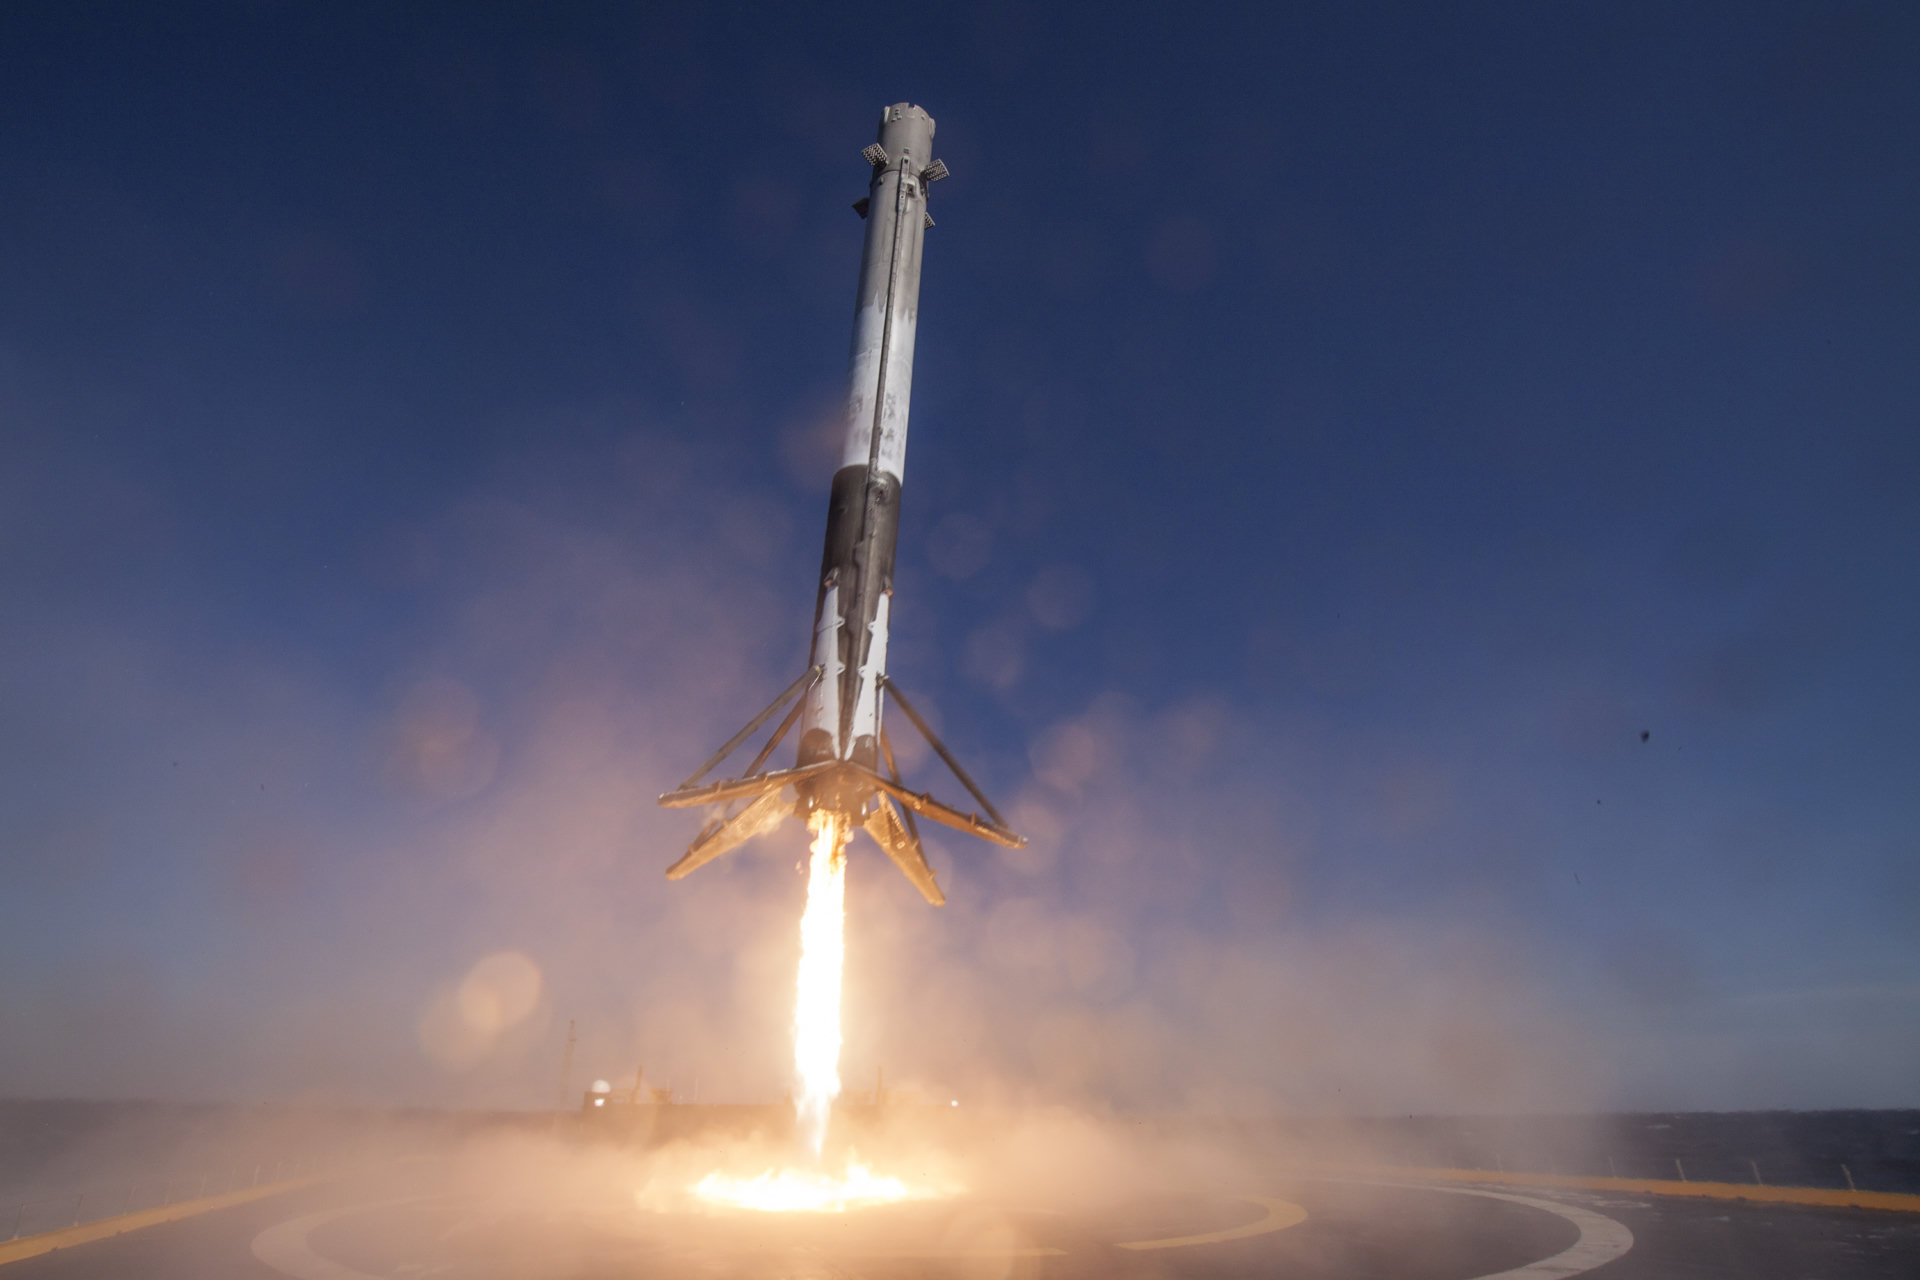
\includegraphics[width=.82\linewidth,height=.30\textheight,keepaspectratio]{figures/booster_photo.jpg}
\caption{A Falcon 9 booster during a powered droneship landing (CRS-8). Photograph: SpaceX, CC0 \cite{photo}. This real recovery example provides context; the seven-engine vehicle studied here is hypothetical.}
\end{figure}
\subsection{Analysis sequence}
The workflow is model specification, finite parameter search, fixed-control replay, and verification. Three clear policies are compared at one initial load before examining sensitivity. Propellant is total methane plus oxygen, with oxygen-to-methane mass ratio 3.4; it is not methane mass alone.
\begin{figure}[htbp]\centering
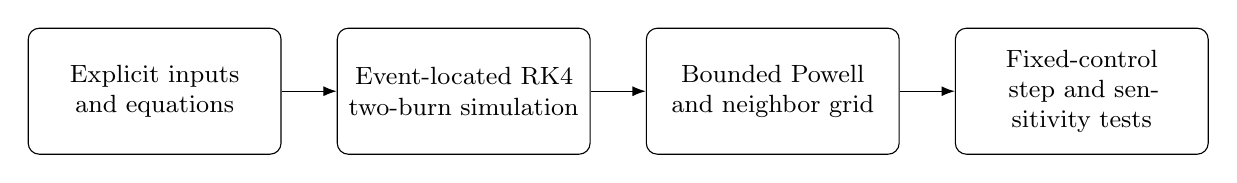
\begin{tikzpicture}[>=Latex,node distance=7mm,box/.style={draw,rounded corners,align=center,font=\small,text width=30mm,minimum height=16mm,inner sep=3pt}]
\node[box](a){Explicit inputs\\and equations};\node[box,right=of a](b){Event-located RK4\\two-burn simulation};\node[box,right=of b](c){Bounded Powell\\and neighbor grid};\node[box,right=of c](d){Fixed-control\\step and sensitivity tests};\draw[->](a)--(b);\draw[->](b)--(c);\draw[->](c)--(d);
\end{tikzpicture}\caption{Computation and verification workflow. The numerical checks do not replace physical calibration.}\end{figure}

\section{Assumptions, Parameters, and Notation}
\subsection{Scope and input classification}
G denotes problem data, P a standard physical relation or atmospheric reference, and H an explicitly chosen modeling assumption. The calculation is planar, with along-track wind and a nonrotating spherical Earth. It does not include lift, cross-track motion, heating, sea-state motion, leg compression, or impact dynamics. Fixed reference area and assumed $C_D(M)$ represent an effective axial drag closure; no calibrated broadside force or moment model is implied.

The $+45^\circ$ initial angle and seven-engine specification are fixed scenario assumptions in addition to the problem geometry and separation speed. The initial flip is idealized before the first powered phase. During thrusting, a bounded first-order axis response represents tracking; it is not a torque-driven rigid-body simulation. A 35 m center-to-foot axial distance and 5 m foot half-span are H geometry. The 35 m distance exceeds the 32.5 m body half-length, leaving 2.5 m nominal axial clearance at vertical first contact. The ship is placed at the nominal contact range; position guidance toward a fixed ship is not modeled.
\begin{table}[htbp]\centering\small\caption{Primary physical and engine inputs.}\label{tab:inputs}
\begin{tabularx}{\linewidth}{@{}lXl@{}}\toprule Quantity & Value & Class\\\midrule
Dry mass; body dimensions & 130,000 kg; 65 m by 7 m & G\\
Initial altitude and speed & 70 km; 1,666.667 m/s & G\\
Initial flight-path angle & $+45^\circ$ & H\\
Engine count; nominal thrust per engine & 7; 1 MN & H\\
Specific impulse; mixture ratio & 330 s; oxygen/methane $=3.4$ & H\\
Earth radius; gravity parameter & $6.371\times10^6$ m; $3.986004418\times10^{14}$ m$^3$/s$^2$ & P\\
Standard gravity; air gas constant & 9.80665 m/s$^2$; 287.05287 J/(kg K) & P\\
Air heat-capacity ratio & 1.4 & H\\
Throttle command range & 0.30--1.10 per enabled engine & H\\
Ignition delay; active response time & 0.5 s; 0.1 s & H\\
Throttle rate; axis lag/rate bound & 1 s$^{-1}$; 1 s and $5^\circ$/s & H\\
Upper-atmosphere scale height & 7,000 m above 86,000 m & H\\
Foot axial reach; half-span & 35 m; 5 m & H\\
\bottomrule\end{tabularx}\end{table}
\subsection{Notation}
\begingroup\small
\begin{longtable}{@{}p{.18\linewidth}p{.76\linewidth}@{}}
\caption{Each model symbol and its meaning.}\\\toprule Symbol & Meaning\\\midrule\endfirsthead
\toprule Symbol & Meaning (continued)\\\midrule\endhead\bottomrule\endfoot
$s$ & Surface range from the separation projection\\
$h$ & Center-of-mass altitude\\
$r$ & Geocentric radius $R_E+h$\\
$u$ & Ground velocity along the local tangent\\
$w$ & Ground vertical velocity, positive upward\\
$m$ & Total vehicle mass\\
$m_{used}$ & Consumed total propellant\\
$m_{res}$ & Residual total propellant\\
$V_g$ & Ground-speed magnitude\\
$V_{rel}$ & Air-relative speed\\
$\rho$ & Air density\\
$C_D$ & Effective axial drag coefficient\\
$M$ & Air-relative Mach number\\
$q$ & Dynamic pressure\\
$p_D$ & Drag per unit reference area\\
$A$ & Fixed reference area $\pi d^2/4$\\
$\phi$ & Thrust-axis angle from the local horizontal\\
$\theta$ & Axis tilt from upward vertical, $\phi-\pi/2$ wrapped to $[-\pi,\pi]$\\
$a$ & Actual common throttle of enabled engines\\
$N$ & Number of enabled engines\\
$T$ & Actual scalar thrust\\
$\vct F_D$ & Aerodynamic drag vector\\
$n_\Sigma$ & Non-gravitational acceleration divided by $g_0$\\
$h_e$ & Entry ignition-request altitude\\
$v_{cut}$ & Entry cutoff air-relative speed\\
$k$ & Stopping-distance multiplier\\
$V_{td}$ & Terminal speed target\\
$z$ & Remaining nominal vertical foot clearance, regularized in guidance\\
$J$ & Dimensionless search objective\\
\end{longtable}\endgroup

\section{Physical Model and Two-Burn Control}
\subsection{Curved-Earth variable-mass translation}
With $r=R_E+h$ and $g(h)=\mu/r^2$, the local-velocity equations retain the basis-curvature terms:
\begin{equation}\begin{aligned}
\dot s&=R_Eu/r,&\dot h&=w,\\
\dot u&=(T\cos\phi+F_{D,x})/m-uw/r,\\
\dot w&=(T\sin\phi+F_{D,z})/m-g(h)+u^2/r.
\end{aligned}\label{eq:motion}\end{equation}
The $-uw/r$ and $u^2/r$ terms are essential to the vacuum angular-momentum and energy checks. The force convention carries drag signs in the vector itself:
\begin{equation}
\vct v_{rel}=(u-W(h),w),\quad q=\tfrac12\rho V_{rel}^2,\quad
\vct F_D=-qC_D(M)A\frac{\vct v_{rel}}{V_{rel}}.
\label{eq:drag}\end{equation}
The zero-speed limit gives zero drag. The reference area is 38.4845 m$^2$; its convention is fixed throughout \cite{drag}.

\subsection{Fully specified atmosphere, wind, and drag}
Below 86 km the model follows the layered hydrostatic relations of USSA 1976 \cite{ussa}. The geopotential radius is $R_a=6356766$ m. Sea-level temperature and pressure are 288.15 K and 101325 Pa. Layer bases in geopotential meters are $0,11000,20000,32000,47000,51000,71000,84852$, with corresponding lapse rates $-0.0065,0,0.001,0.0028,0,-0.0028,-0.002$ K/m. The capped geopotential coordinate and upper continuation are
\begin{equation}\begin{aligned}
H&=\min\!\left(\frac{R_ah}{R_a+h},84852\right),\qquad
\rho=\frac{p}{R_{air}T_a},\\
\rho(h>86000)&=\rho(86000)\exp\!\left[-\frac{h-86000}{7000}\right],\qquad
c(h>86000)=c(86000).
\end{aligned}\label{eq:atmosphere}\end{equation}
Within each lower layer, $T_a=T_b+L_b(H-H_b)$, and the pressure ratio is $\exp[-g_0(H-H_b)/(R_{air}T_b)]$ for $L_b=0$, or $(T_b/T_a)^{g_0/(R_{air}L_b)}$ otherwise. Sound speed is $c=\sqrt{1.4R_{air}T_a}$. The 7 km continuation is an H extrapolation, not the full upper USSA model. Its 5 and 10 km alternatives are tested separately.

\begin{table}[htbp]
\centering\small
\caption{All 12 assumed axial drag anchors (H).}
\label{tab:cd}
\begin{tabularx}{\linewidth}{@{}rX@{}}
\toprule
Mach & $C_D$ \\
\midrule
0.00 & 0.50 \\
0.30 & 0.50 \\
0.60 & 0.55 \\
0.80 & 0.75 \\
0.95 & 1.10 \\
1.00 & 1.35 \\
1.10 & 1.50 \\
1.30 & 1.35 \\
1.60 & 1.15 \\
2.00 & 1.00 \\
3.00 & 0.85 \\
8.00 & 0.75 \\
\bottomrule
\end{tabularx}
\par\smallskip{\footnotesize Piecewise-linear interpolation in Mach; endpoint values are held outside the tabulated domain. These are declared assumptions, not recovered or measured booster data.}
\end{table}

\begin{table}[htbp]
\centering\small
\caption{Prescribed along-track wind profile (H).}
\label{tab:wind}
\begin{tabularx}{\linewidth}{@{}rX@{}}
\toprule
Altitude (km) & Wind (m/s) \\
\midrule
0 & 8 \\
2 & 8 \\
6 & 16 \\
12 & 35 \\
20 & 20 \\
35 & 5 \\
70 & 0 \\
200 & 0 \\
\bottomrule
\end{tabularx}
\par\smallskip{\footnotesize Piecewise-linear interpolation; no vertical wind or cross-track motion is represented.}
\end{table}

The twelve coefficients in \cref{tab:cd} are deliberately explicit assumptions for this hypothetical booster. They are not wind-tunnel or CFD measurements. Linear interpolation uses every anchor, with no hidden smoothing. The wind in \cref{tab:wind} is prescribed along track and constant in time; the 8 m/s surface value represents a sea-wind scenario rather than measured weather.

\subsection{Engine and axis response}
For nominal per-engine thrust $T_e=10^6$ N,
\begin{equation}
T=NT_ea,\qquad \dot m=-\frac{T}{I_{sp}g_0},\qquad
m_{CH_4}=m_{used}/4.4,\quad m_{O_2}=3.4m_{used}/4.4.
\label{eq:mass}\end{equation}
The effective exhaust speed is $I_{sp}g_0$ \cite{isp}. Ignition requests precede actual thrust by 0.5 s. Enabled-engine response and axis tracking are
\begin{equation}
\dot a=\operatorname{clip}\!\left(\frac{a_c-a}{0.1},-1,1\right),\qquad
\dot\phi=\operatorname{clip}\!\left(\frac{\operatorname{wrap}(\phi_c-\phi)}{1\ \mathrm{s}},-5^\circ/\mathrm{s},5^\circ/\mathrm{s}\right).
\label{eq:actuator}\end{equation}
The command $a_c$ lies in $[0.3,1.1]$ while engines are enabled; startup actual throttle can be below 0.3. Shutdown is instantaneous in this model. At a reduction of engine count the remaining engines retain their actual throttle and then respond through \cref{eq:actuator}; there is no instantaneous compensating throttle increase.

Seven engines operate during entry. During terminal braking, seven reduce to three when CM altitude is below 15 km, requested thrust below 3.05 MN, and actual thrust below 3.1 MN. Three reduce to two below 2 km, with corresponding thresholds 2.05 and 2.1 MN. These are specified control rules, not an optimized discrete engine sequence. One engine at 1.1 MN is below the 1.275 MN dry weight, whereas two or three offer terminal support; the final choice also depends on transient braking and throttle floor.

\subsection{Contact geometry and ignition triggers}
For H foot geometry $\ell=35$ m, $b=5$ m, geometric first contact occurs at
\begin{equation}
 h_c(\theta)=\ell\cos\theta+b|\sin\theta|,\qquad h-h_c=0.
\label{eq:contact}\end{equation}
This is a kinematic contact event, not a leg-impact simulation. The initial ship position is free and chosen at the nominal surface range.

Entry is requested on descent through $h_e$. After delay, seven engines fire opposite relative airflow until $V_{rel}\le v_{cut}$. Policy S0 instead cuts off at 55 km. The terminal request uses either stopping distance or drag loading:
\begin{equation}
 h-h_c\le k\frac{\max(V_g^2-V_{td}^2,0)}{2\max(7T_ea_{max}/m-g,0.01\ \mathrm{m/s^2})}.
\label{eq:stopping}\end{equation}
\begin{equation}
p_D\equiv\frac{|\vct F_D|}{A}=qC_D,\qquad
p_D\ge25000\ \mathrm{Pa} \Longleftrightarrow\
V_{rel}\ge\sqrt{\frac{2(25000\ \mathrm{Pa})}{\rho C_D}}.
\label{eq:dragtrigger}\end{equation}
Thus \cref{eq:dragtrigger} is explicitly a \emph{drag-loading trigger}. The denominator contains $C_D$ because the bounded quantity is $D/A$, not $q$. A pure dynamic-pressure trigger would have no $C_D$ in its denominator. The 25 kPa drag-loading threshold is distinct from the 50 kPa dynamic-pressure acceptance limit. A further pressure-protection mode requests maximum enabled-engine thrust when $q$ crosses 35 kPa upward and releases on a downward crossing; both crossings are located as events. None of these rules alone guarantees the future pressure peak; acceptance uses the computed maximum.

\subsection{Terminal force law and load screen}
Let $z=\max(h-h_c,0.5\ \mathrm{m})$ and $t_g=\max[2z/(\max(-w,0)+V_{td}),0.5\ \mathrm{s}]$. The desired local acceleration terms are
\begin{equation}\begin{aligned}
a_{x,g}&=-2u/t_g+uw/r,\\
a_{z,g}&=\frac{-w|w|-V_{td}^2}{2z}+g-u^2/r.
\end{aligned}\label{eq:guidance}\end{equation}
The sign $-w|w|$ changes the vertical correction if the vehicle begins ascending. The 0.5 m guidance floor regularizes the terminal law and is independent of integration step size.
\begin{equation}
\vct F_{req}=m(a_{x,g},a_{z,g})-\vct F_D,\qquad
T_{req}=|\vct F_{req}|,\quad
\phi_c=\operatorname{clip}\{\arg\vct F_{req},\pi/2-\theta_c,\pi/2+\theta_c\}.
\label{eq:force}\end{equation}
Here $\theta_c=[2+58\min(z/5000,1)]^\circ$. The requested magnitude is limited by engine capacity and a 3.7 $g_0$ resultant-load control margin. With $\vct n_c=(\cos\phi_c,\sin\phi_c)$ and $P=\vct F_D\cdot\vct n_c$, the nonnegative cap is $\max\{0,-P+\sqrt{\max[0,(3.7mg_0)^2-|\vct F_D|^2+P^2]}\}$. Actual load is evaluated using the lagged applied direction: $n_\Sigma=|T(\cos\phi,\sin\phi)+\vct F_D|/(mg_0)$. Consequently, pressure and load are coupled through the aerodynamic force.

A passing screen has geometric contact before 900 s, no fuel exhaustion, downward speed at most 2.5 m/s, $|u_f|\le1$ m/s, $|\theta_f|\le2^\circ$, $q_{max}\le50$ kPa, $n_{max}\le4$, and residual propellant at least 1,000 kg. These are H screens, not material-strength or sea-state certification.

\subsection{Numerical and modeling choices}
The five physical/control states plus axis and throttle states form a small nonstiff system; four additional states integrate local thrust components for the burn-force report. Classical RK4 is transparent and fourth order for a smooth right-hand side \cite{hairer}. The complete system is hybrid: ignition, cutoff, staging, pressure protection, and contact alter the active equations. For each smooth substep, $k_1=f(t,y)$, $k_2=f(t+\Delta t/2,y+\Delta t k_1/2)$, $k_3=f(t+\Delta t/2,y+\Delta t k_2/2)$, $k_4=f(t+\Delta t,y+\Delta t k_3)$ and $y^+=y+\Delta t(k_1+2k_2+2k_3+k_4)/6$. Every discrete guard crossing is located with 30 bisections of an RK4 substep. Pressure and load maxima are sampled over accepted step and event states; no interpolated peak fit is used. Saturation corners and peak sampling still prevent an automatic fourth-order claim for all output metrics. The actual step test appears in \cref{sec:verification}.

The initial flip, fixed effective drag area, wind, and simplified axis tracking make a tractable screening model. Variable mass, altitude-dependent gravity and curvature remain because their effects are not uniformly small. This hierarchy is sufficient to compare policies under identical stated assumptions; it does not resolve full six-degree-of-freedom stability or heating.

\section{Search Domain and Dimensionless Objective}
\begin{table}[htbp]
\centering\small
\caption{Search domain, normalized parameter coordinates, and selected control.}
\label{tab:search_domain}
\begin{tabularx}{\linewidth}{@{}lXX@{}}
\toprule
Variable & Range & Selected \\
\midrule
$h_e$ (km) & 35--82 & 57.616426 \\
$v_{cut}$ (m/s) & 450--1150 & 897.178136 \\
$k$ & 0.95--1.60 & 1.59749787 \\
$V_{td}$ (m/s) & 0.5--2.0 & 1.33272273 \\
\bottomrule
\end{tabularx}
\par\smallskip{\footnotesize Full-precision selected.json supplies the fixed control vector in the step study. The finite search does not certify global optimality.}
\end{table}

Entry heights bracket earlier and later braking. The cutoff-speed interval permits long or short entry pulses, and $k$ spans cautious and less cautious stopping-distance triggers. The target-speed range stays below the 2.5 m/s acceptance speed but allows actuator response to affect actual contact speed. These ranges are H exploratory bounds, not proof that all feasible solutions are contained within them.

Powell is itself an optimizer. Its derivative-free search avoids reliance on gradients through phase changes, force saturation, and fuel exhaustion \cite{powell,scipy}. The implementation evaluates 18 deterministic initial grid points, takes the best three starts into bounded Powell runs, and applies an ordered 27-neighbor refinement. Powell uses at most 35 iterations and 800 evaluations per start, with \texttt{xtol}=0.001 and \texttt{ftol}=$10^{-5}$. Status and evaluation counts are retained, including any budget-limited run. Parameter coordinates are $z_i=(p_i-p_{i,min})/(p_{i,max}-p_{i,min})\in[0,1]$.

\begin{equation}
J=\frac{m_{used}}{100000\ \mathrm{kg}}+1000\sum_{i=1}^{7}r_i^2.
\label{eq:objective}\end{equation}
\begin{table}[htbp]
\centering\small
\caption{Dimensionless penalties and separate acceptance limits.}
\label{tab:penalty}
\begin{tabularx}{\linewidth}{@{}lXlX@{}}
\toprule
Channel & Design scale & $r_i$ & Acceptance \\
\midrule
Downward speed & 2.2 m/s & $[-w_f/2.2-1]_+$ & 2.5 m/s \\
Upward velocity & 2.2 m/s & $[w_f/2.2]_+$ & $w_f\le0$ \\
Horizontal speed & 0.8 m/s & $[|u_f|/0.8-1]_+$ & 1.0 m/s \\
Peak pressure & 47.5 kPa & $[q_{max}/47500-1]_+$ & 50 kPa \\
Load factor & 3.9 & $[n_{max}/3.9-1]_+$ & 4.0 \\
Final tilt & $1.8^\circ$ & $[|\theta_f|/1.8^\circ-1]_+$ & $2^\circ$ \\
Residual propellant & 1500 kg & $[(1500-m_{res})/1500]_+$ & 1000 kg \\
\bottomrule
\end{tabularx}
\par\smallskip{\footnotesize $[x]_+=\max(x,0)$. Pressure in the residual is expressed in Pa; angles use the displayed degree ratio. The mass scale is $m_*=100000$ kg, the common penalty weight is 1000, and a no-contact run receives $10^8+m_{used}/m_*$.}
\end{table}

\FloatBarrier
All seven residuals in \cref{tab:penalty} are dimensionless, so \cref{eq:objective} adds quantities with consistent normalization. A no-contact trajectory has objective $10^8+m_{used}/m_*$, with $m_*=100000$ kg. Soft design targets differ deliberately from acceptance. A low objective does not replace the independent pass/fail screen. CasADi/IPOPT is not used here, and a bounded finite search is not an unrestricted optimal-control solution.

The load loop starts at 90 t and increments by 10 t, re-searching the four parameters at each load. The first passing tested load ends the loop. A failed search at a lighter load does not prove that load infeasible under all controls.

\section{Newly Computed Return and Two-Burn Budget}
\subsection{Load search and policy comparison}
\begin{table}[htbp]
\centering\small
\caption{Sequential 10 t load search; each row has its own searched control.}
\label{tab:scan}
\begin{tabularx}{\linewidth}{@{}rrrrrX@{}}
\toprule
Load (t) & Used (t) & Entry (t) & Terminal (t) & $q_{max}$ (kPa) & Outcome \\
\midrule
90 & 90.000 & 56.641 & 33.359 & 102.59 & Fail \\
100 & 98.620 & 60.188 & 38.432 & 96.49 & Fail \\
110 & 108.600 & 63.990 & 44.611 & 84.15 & Fail \\
120 & 118.577 & 68.116 & 50.461 & 68.96 & Fail \\
130 & 128.078 & 71.374 & 56.704 & 45.94 & Pass \\
\bottomrule
\end{tabularx}
\par\smallskip{\footnotesize Search uses 0.1 s and validation 0.02 s. Failed rows show consumption before contact or exhaustion, not the fuel required for a successful terminal burn. Failure details and every row's parameters are retained in \texttt{load\_search.json}.}
\end{table}

\begin{table}[htbp]
\centering\small
\caption{Three strategies at the selected initial load, all replayed at 0.005 s.}
\label{tab:strategy}
\begin{tabularx}{\linewidth}{@{}lrrrrX@{}}
\toprule
Policy & Entry (t) & Terminal (t) & $|w_f|$ (m/s) & $q_{max}$ (kPa) & Screen \\
\midrule
S0 & 38.828 & 91.172 & 253.543 & 39.45 & Fail \\
S1 & 77.929 & 52.071 & 45.505 & 53.63 & Fail \\
S2 & 71.374 & 56.704 & 2.203 & 45.94 & Pass \\
\bottomrule
\end{tabularx}
\par\smallskip{\footnotesize S0: entry from 75 to 55 km, k=1.30 and target 1.50 m/s; S1: 75 km entry with a 750 m/s cutoff, k=1.40 and target 1.50 m/s; S2: searched parameters in the search-domain table. All three use the same environment, actuator model, acceptance screen, and terminal law.}
\end{table}

The first passing load found is \RLoad{} t. Failure reasons, controls, and objective statuses accompany each row in the machine-readable results. The comparison uses the same total load for all three policies; changing only burn timing or cutoff can still exhaust the same fuel supply. The terminal columns include failed attempts as explicitly labeled. No minimum--maximum range is formed by mixing successful burns and fuel-exhausted runs.
\begin{figure}[htbp]\centering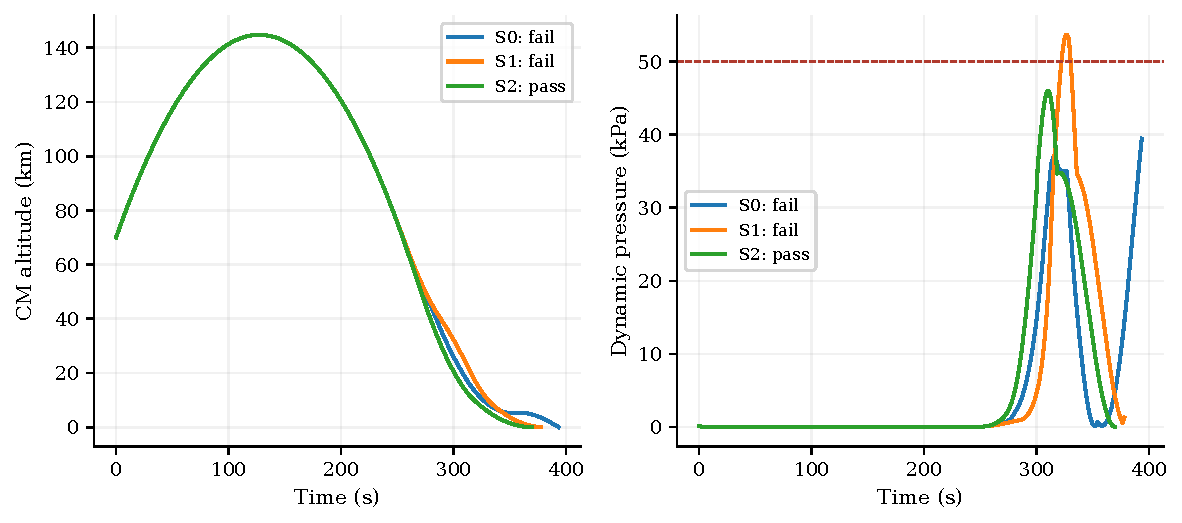
\includegraphics[width=\linewidth]{strategies.pdf}\caption{The three actual policy runs at the selected load. Failed cases remain visible. The dashed pressure line is the 50 kPa acceptance limit.}\end{figure}
\subsection{Trajectory and stage sequence}
\begin{figure}[htbp]\centering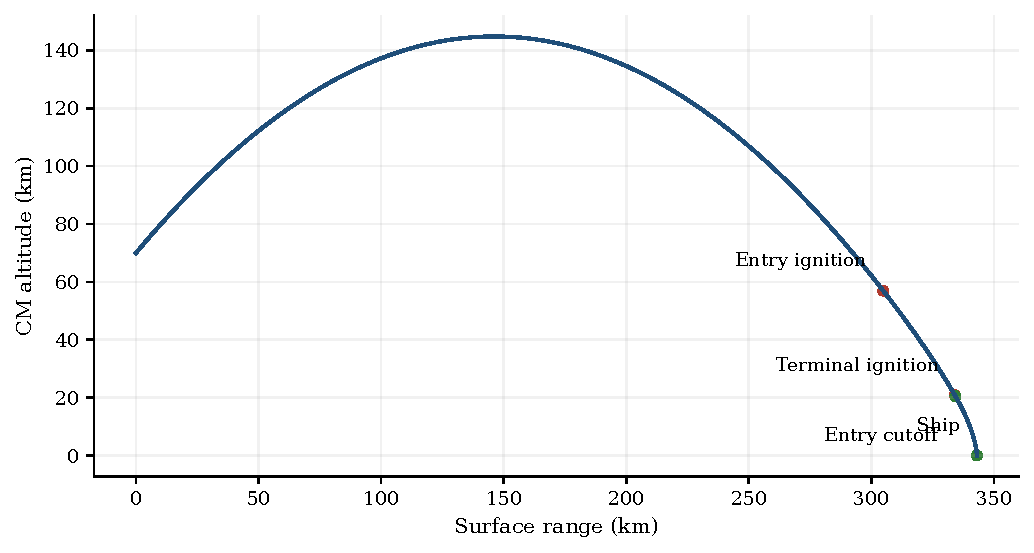
\includegraphics[width=\linewidth]{trajectory.pdf}\caption{Computed CM altitude against surface range for the selected policy. Marker locations are taken from the event-located solution.}\end{figure}
The nominal apogee is \RApogee{} km. The ship is placed near surface range \RRange{} km, where contact occurs at \RTf{} s. The vehicle first coasts upward and returns, then performs an entry pulse, an ignition-delay transition, and terminal braking. In the selected case, the terminal request coincides with entry cutoff; the 0.5 s restart delay separates the two thrust-on intervals. There are two thrust-on phases; subsequent reductions of enabled engines do not constitute a third ignition.
\begin{figure}[htbp]\centering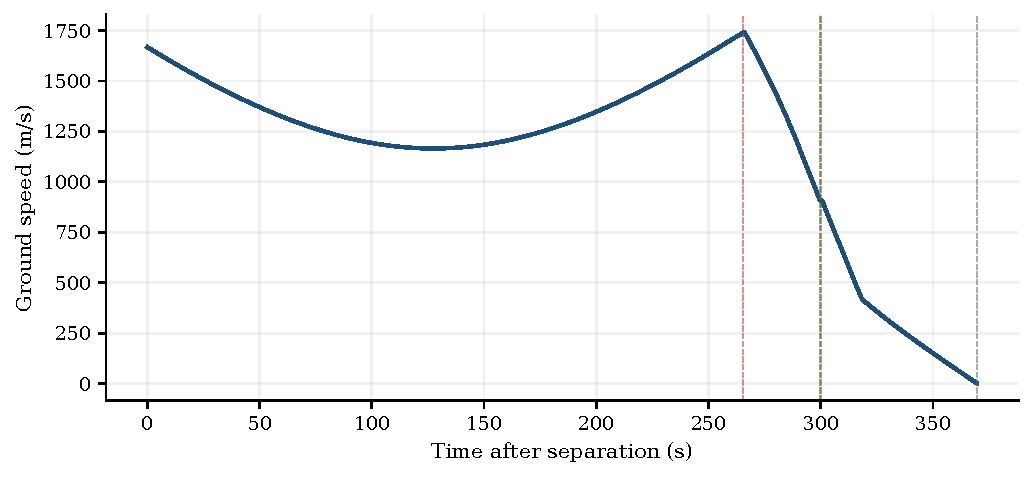
\includegraphics[width=\linewidth]{speed.pdf}\caption{Computed ground-speed history. Dashed markers denote entry start/cutoff, terminal start, and contact.}\end{figure}
\begin{figure}[htbp]\centering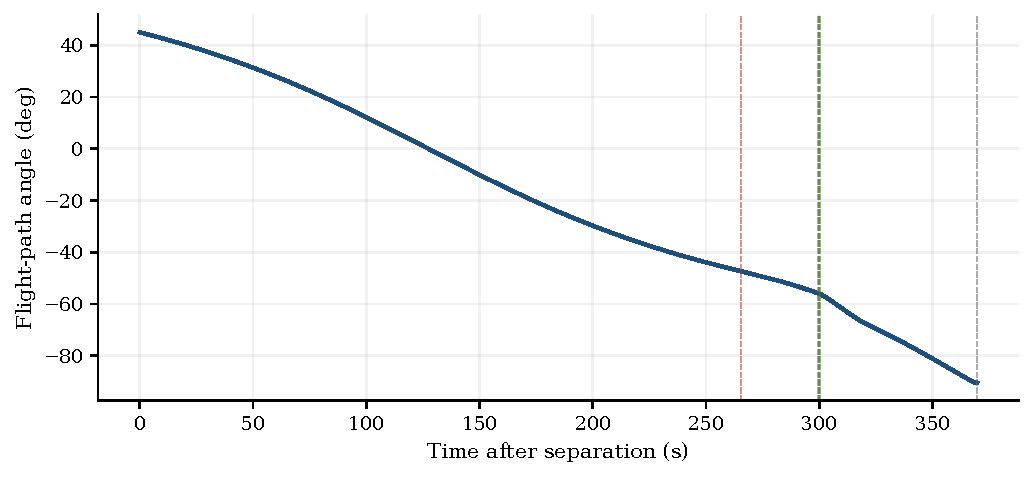
\includegraphics[width=\linewidth]{gamma.pdf}\caption{Flight-path angle $\operatorname{atan2}(w,u)$. It describes ground velocity, not body-axis orientation.}\end{figure}
\begin{figure}[htbp]\centering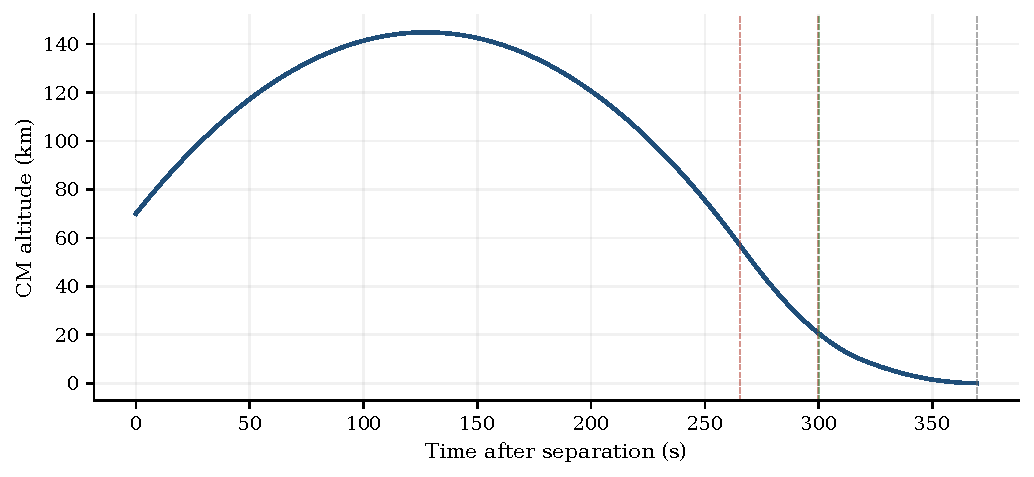
\includegraphics[width=\linewidth]{height.pdf}\caption{CM altitude history. Contact occurs at the finite CM height defined by the foot geometry, rather than at $h=0$.}\end{figure}
\subsection{Fuel species and applied force}
\begin{table}[htbp]
\centering\small
\caption{Propellant species and scalar thrust for the two powered phases.}
\label{tab:burns}
\begin{tabularx}{\linewidth}{@{}lrrrrX@{}}
\toprule
Burn & Total (t) & CH$_4$ (t) & O$_2$ (t) & Duration (s) & Mean/peak (MN) \\
\midrule
Entry & 71.374 & 16.221 & 55.153 & 34.239 & 6.746 / 7.000 \\
Terminal & 56.704 & 12.887 & 43.817 & 69.450 & 2.642 / 5.625 \\
\bottomrule
\end{tabularx}
\par\smallskip{\footnotesize The oxygen-to-methane mass ratio is 3.4. Mean scalar thrust equals $m_{used} I_{sp}g_0/\Delta t$. Counts during terminal braking are selected by the explicit 7-to-3-to-2 guards; shutdown is idealized as instantaneous.}
\end{table}

\begin{table}[htbp]
\centering\small
\caption{Mean local thrust components, computed from integrated applied force.}
\label{tab:force}
\begin{tabularx}{\linewidth}{@{}lrrX@{}}
\toprule
Burn & $\overline T_x$ (MN) & $\overline T_z$ (MN) & Direction \\
\midrule
Entry & -4.216 & 5.257 & Upward and against downrange motion \\
Terminal & -0.919 & 2.400 & Upward and against downrange motion \\
\bottomrule
\end{tabularx}
\par\smallskip{\footnotesize Components refer to the local tangent and upward directions at each instant. They are not a single vector impulse in a fixed inertial frame. Exhaust points opposite the thrust axis.}
\end{table}

The entry pulse consumes \REntryFuel{} t and terminal braking \RTerminalFuel{} t, totaling \RUsed{} t with \RReserve{} t remaining. The table reports only the selected successful case, so its terminal requirement is not confused with consumption truncated by exhaustion. Entry thrust opposes air-relative velocity. Terminal thrust follows the force law, generally upward and against residual downrange motion. The vector means and peak scalar forces are computed from the applied forces rather than nominal engine count alone.
\begin{figure}[htbp]\centering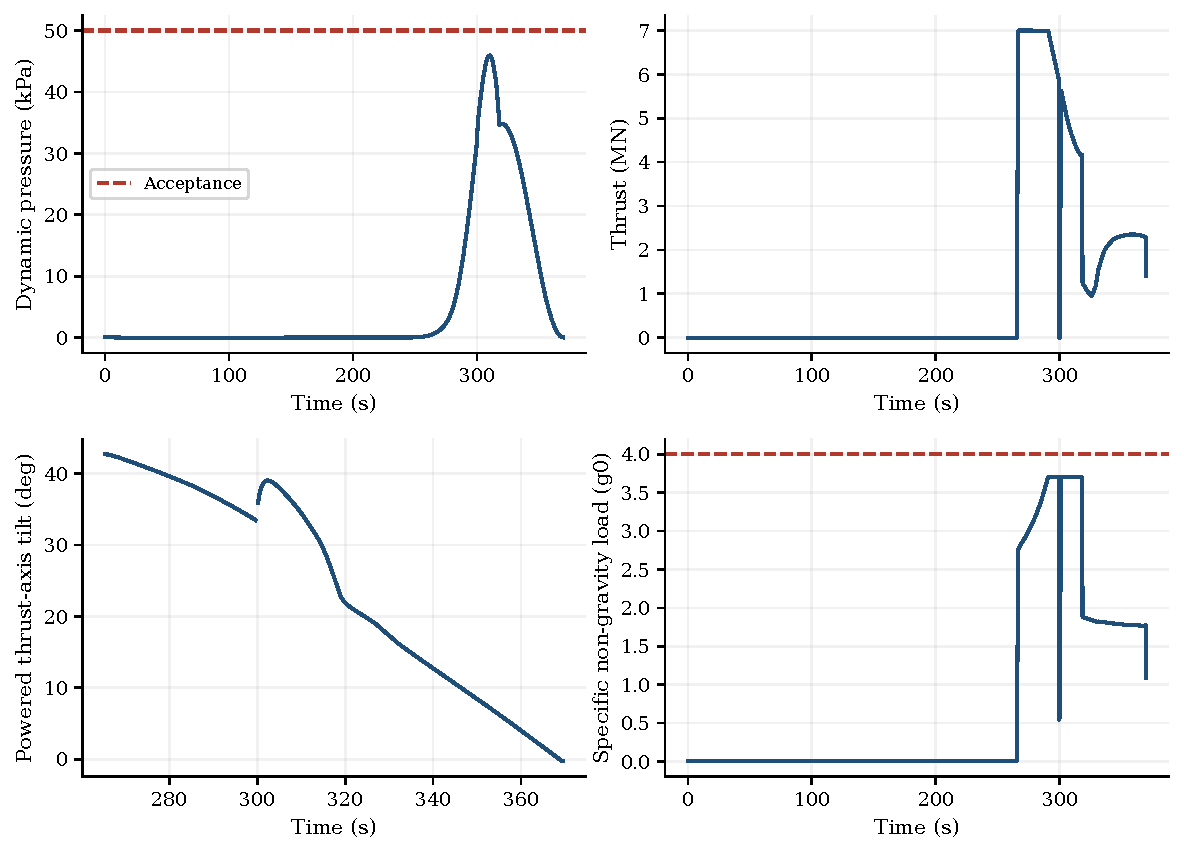
\includegraphics[width=\linewidth]{controls.pdf}\caption{Actual dynamic pressure, thrust, powered-axis tilt and non-gravitational load. Axis values during unpowered coast are omitted because the ideal alignment bookkeeping is not a resolved physical flip trajectory.}\end{figure}

\section{Measured Numerical Verification}\label{sec:verification}
\subsection{Three fixed-control step sizes}
\begin{table}[htbp]
\centering\small
\caption{Actual fixed-control step-halving results; no reoptimization.}
\label{tab:convergence}
\begin{tabularx}{\linewidth}{@{}rrrrr@{}}
\toprule
Step (s) & Consumed (kg) & $|w_f|$ (m/s) & $q_{max}$ (Pa) & Contact time (s) \\
\midrule
0.020 & 128078.233034 & 2.203605464 & 45942.273947 & 369.581277792 \\
0.010 & 128078.262525 & 2.203256744 & 45942.128561 & 369.581324869 \\
0.005 & 128078.246507 & 2.203477993 & 45942.183628 & 369.581304073 \\
\bottomrule
\end{tabularx}
\par\smallskip{\footnotesize Digits expose numerical changes only, not physical accuracy. Every row passes the same nominal acceptance screen. The 0.005 s run supplies the final reported trajectory.}
\end{table}

\begin{table}[htbp]
\centering\small
\caption{Signed differences relative to the 0.005 s run.}
\label{tab:differences}
\begin{tabularx}{\linewidth}{@{}rrrrr@{}}
\toprule
Step (s) & $\Delta m$ (kg) & $\Delta |w_f|$ (m/s) & $\Delta q$ (Pa) & $\Delta t_f$ (ms) \\
\midrule
0.020 & -0.013472 & 0.00012747 & 0.090319 & -0.026281 \\
0.010 & 0.016018 & -0.00022125 & -0.055066 & 0.020797 \\
\bottomrule
\end{tabularx}
\end{table}

\begin{table}[htbp]
\centering\small
\caption{Actual event-time comparison under step halving.}
\label{tab:events}
\begin{tabularx}{\linewidth}{@{}Xrrr@{}}
\toprule
Event & 0.02 s step & 0.01 s step & 0.005 s step \\
\midrule
Entry request & 264.891636490 & 264.891636489 & 264.891636489 \\
Entry thrust begins & 265.391636490 & 265.391636489 & 265.391636489 \\
Entry cutoff & 299.630971081 & 299.630970973 & 299.630970962 \\
Terminal request & 299.630971081 & 299.630970973 & 299.630970962 \\
Terminal thrust begins & 300.130971081 & 300.130970973 & 300.130970962 \\
Pressure override on & 300.738953379 & 300.738956337 & 300.738955479 \\
Pressure override off & 318.134575569 & 318.134513040 & 318.134535141 \\
7 to 3 engines & 318.285945992 & 318.285884085 & 318.285905965 \\
3 to 2 engines & 369.480378970 & 369.480449585 & 369.480418601 \\
Geometric contact & 369.581277792 & 369.581324869 & 369.581304073 \\
\bottomrule
\end{tabularx}
\par\smallskip{\footnotesize All entries are seconds after separation. Crossing guards are located by 30 bisections of a re-integrated RK4 substep; actuator saturation remains piecewise smooth.}
\end{table}

The parameter vector, atmospheric anchors, control rules, and engine settings remain unchanged in all three runs. In particular, no optimization is repeated between step sizes. The fine-pair changes are \RFineDm{} kg in consumption, \RFineDv{} m/s in contact-speed magnitude, \RFineDq{} Pa in peak pressure, and \RFineDt{} ms in contact time. Event times are listed separately in \cref{tab:events}, not inferred from a visually smooth curve.

The changes are not uniformly monotone. Three points therefore support a measured small numerical difference over this range, not a reliable asymptotic order estimate or an error bound on the exact hybrid solution. The formal fourth-order property applies to smooth segments, while switching and saturation can alter output convergence. Every run passes the same nominal acceptance screen.
\subsection{Physical identities and execution record}
With drag and thrust removed, the central-gravity equations conserve $E=(u^2+w^2)/2-\mu/r$ and angular momentum per mass $H=ru$. The recorded relative drifts are below $10^{-12}$, with exactly constant mass. The nominal calculation also has nonpositive drag power $\vct F_D\cdot\vct v_{rel}$, exact numerical mass-budget closure to the stored precision, and measured active-engine throttle slew consistent with 1 s$^{-1}$. These checks verify implementation identities rather than uncertain aerodynamic coefficients.

\begin{table}[htbp]
\centering\small
\caption{Measured numerical identity checks.}
\label{tab:identities}
\begin{tabularx}{\linewidth}{@{}Xrl@{}}
\toprule
Check & Measured value & Criterion \\
\midrule
Vacuum energy relative drift & 2.463e-16 & $<10^{-9}$ \\
Vacuum angular-momentum drift & 4.146e-15 & $<10^{-9}$ \\
Vacuum mass change (kg) & 0.000e+00 & $<10^{-8}$ \\
Smooth-interval mass-flow residual (kg) & 0.012885 & $<0.1$ in magnitude \\
Active-engine throttle slew (1/s) & 1.000000000 & $\le1+10^{-6}$ \\
\bottomrule
\end{tabularx}
\par\smallskip{\footnotesize The mass-flow residual compares state mass loss with an independent trapezoidal integral of recorded scalar thrust divided by $I_{sp}g_0$, excluding discontinuous phase/count boundaries.}
\end{table}

The electronic archive contains \texttt{config.json}, the complete C++ kernel and Python search, plotting, and report scripts, frozen controls, full-precision CSV/JSON outputs, compressed trajectories, logs, and a compiler/dependency manifest. The command \texttt{python simulation/reproduce.py --latex} reconstructs the study and document. The five appendix pages show code actually used by this pipeline; omitted support files are supplied unabridged electronically. No illustrative substitute is presented as the generator of these tables.

\section{Sensitivity and Landing Interpretation}
\begin{table}[htbp]
\centering\small
\caption{Fixed-control perturbations at the selected load.}
\label{tab:sensitivity}
\begin{tabularx}{\linewidth}{@{}Xrrrrl@{}}
\toprule
Change & Used (t) & $|w_f|$ (m/s) & $q_{max}$ (kPa) & $\Delta s$ (m) & Screen \\
\midrule
Cd -10\% & 129.773 & 2.229 & 46.61 & 32.0 & Fail \\
Cd +10\% & 126.546 & 2.184 & 45.49 & -34.8 & Pass \\
Wind x1.25 & 128.004 & 2.197 & 45.56 & 1.5 & Pass \\
Isp -2\% & 129.755 & 2.226 & 45.55 & -12.9 & Fail \\
Ignition delay 0.7 s & 127.778 & 2.200 & 49.55 & 69.0 & Pass \\
Upper scale 5 km & 128.078 & 2.203 & 45.94 & 0.7 & Pass \\
Upper scale 10 km & 128.078 & 2.203 & 45.94 & -1.2 & Pass \\
\bottomrule
\end{tabularx}
\par\smallskip{\footnotesize The screen tests velocity, load, tilt and fuel, not a fixed-ship position constraint. Range shifts are measured relative to the nominal ship location; passing the screen does not establish robust deck capture.}
\end{table}

Control parameters are frozen during every perturbation. A lower drag coefficient or lower specific impulse can consume the reserve and fail the screen, even when the numerical step changes are much smaller. Increasing the upper scale height from 7 km changes only the extremely thin portion of the early arc in these cases. This does not validate the extrapolation against actual upper-atmosphere weather.

The ship is placed for the nominal trajectory. The range shifts in \cref{tab:sensitivity} show why velocity control alone is not robust fixed-deck position control. A passing perturbation flag screens speeds, tilt, loads and reserve only. Deck motion, cross-track winds, position feedback, leg forces, post-contact thrust cutoff and tipping remain outside the demonstrated result.

\section{Discussion of Reliability and Limitations}
Numerical reproducibility is now closed at the level of the stated equations and supplied inputs: every coefficient, interpolation rule, control branch and objective scale is explicit, and all displayed trajectories and numerical tables are computed. This is a different claim from proving that the drag law, engine assumptions, or geometry represent a particular operational rocket.

The axial drag anchors are assumed. Fixed reference area suppresses uncalibrated attitude--aerodynamic force and moment coupling; the axis response is not a rigid-body controller. A $2^\circ$ contact tilt screen does not demonstrate that required moments or leg-load limits are attainable. The nominal reserve screen also does not cover arbitrary weather or engine-out behavior. The sensitivity failures are material limitations of the candidate, not numerical defects hidden by rounding.

The first passing 10 t load and a local bounded search give a conditional design point. They do not establish a continuous minimum, uniqueness, or a failure probability. Additional calibration and six-degree-of-freedom guidance and contact models would change the interpretation of physical safety, even if the present numerical verification remained intact.

\section{Conclusion}
Under the explicit new assumptions, the first nominally passing load found is \RLoad{} t. The selected return consumes \RUsed{} t, split into \REntryFuel{} t entry and \RTerminalFuel{} t terminal propellant, and leaves \RReserve{} t. Contact downward speed is \RWf{} m/s, with peak dynamic pressure \RQmax{} kPa and peak specific non-gravitational load \RNmax{} $g_0$.

Three actual fixed-control step sizes and event-time comparisons show small integration differences at the tested resolutions. Complete scripts and inputs generate the results; the twelve drag anchors, 7 km density continuation and dimensionless objective are exposed rather than inferred. Parameter sensitivity remains more significant than the fine-step numerical differences. The candidate is reproducible and nominally feasible for this screening model, with physical recovery reliability still conditional on the stated approximations.

\section{AI Usage Report}
\subsection{System Used}
OpenAI ChatGPT with Codex tools was used during preparation of the study; an exact deployed model identifier is not available in the retained record.
\subsection{Scope and Nature of Use}
AI assistance included model formulation, implementation of the C++/Python pipeline, debugging of event and actuator logic, literature lookup, numerical testing, data analysis, plotting, academic editing and LaTeX preparation. These contributions extend beyond language correction. The recovery photograph was extracted from the uploaded archive without image synthesis or retouching.
\subsection{Content Authorship}
The numerical tables in this revision were produced by executing the supplied implementation under the declared assumptions. The numerical inputs and their assumptions are explicit in the accompanying configuration. AI-assisted code and explanations are disclosed as such; this statement does not assert independent human authorship of every equation or algorithm. Team 856 is responsible for the interpretation and submission. The record format follows the competition disclosure rules \cite{rules}.
\subsection{Quality Assurance}
Actual checks comprise fixed-control step halving, vacuum invariants, drag-power sign, mass closure, throttle slew, event timing, and deterministic perturbations. The checks support the numerical claims made here and do not certify flight hardware. Retained exchanges, source files, outputs and execution logs are archived in the accompanying electronic materials.

\clearpage\phantomsection\addcontentsline{toc}{section}{References}
\begin{thebibliography}{8}\small
\bibitem{ussa} NOAA/NASA/USAF. \emph{U.S. Standard Atmosphere, 1976}. NASA-TM-X-74335, 1976. \url{https://ntrs.nasa.gov/citations/19770009539}.
\bibitem{drag} NASA Glenn Research Center. \emph{Drag Equation}. \url{https://www1.grc.nasa.gov/beginners-guide-to-aeronautics/drag-equation/}.
\bibitem{isp} NASA Glenn Research Center. \emph{Specific Impulse}. \url{https://www1.grc.nasa.gov/beginners-guide-to-aeronautics/specific-impulse/}.
\bibitem{powell} M. J. D. Powell. An efficient method for finding the minimum of a function of several variables without calculating derivatives. \emph{The Computer Journal}, 7(2):155--162, 1964. DOI: \url{https://doi.org/10.1093/comjnl/7.2.155}.
\bibitem{scipy} SciPy Developers. \emph{minimize(method='Powell')}. \url{https://docs.scipy.org/doc/scipy/reference/optimize.minimize-powell.html}.
\bibitem{hairer} E. Hairer, S. P. N\o rsett, and G. Wanner. \emph{Solving Ordinary Differential Equations I}. 2nd ed., Springer, 1993. DOI: \url{https://doi.org/10.1007/978-3-540-78862-1}.
\bibitem{photo} SpaceX. \emph{CRS-8 first stage landing}, photograph, CC0. \url{https://commons.wikimedia.org/wiki/File:CRS-8_first_stage_landing_(25787998624).jpg}.
\bibitem{rules} University Physics Competition. \emph{Contest Rules}. \url{https://www.uphysicsc.com/contestrules.html}.
\end{thebibliography}
\clearpage\appendix\section{Executed Implementation Listings}\label{app:code}
\noindent These five pages print files or marked excerpts actually used to generate the new study. The complete kernel and support files accompany the electronic archive; these printed selections are not a standalone reduced model.
\lstset{basicstyle=\ttfamily\fontsize{8}{9}\selectfont,keywordstyle=\mdseries,commentstyle=\mdseries,stringstyle=\mdseries,numbers=left,numberstyle=\tiny,numbersep=5pt,frame=single,breaklines=true,columns=fullflexible,keepspaces=true,showstringspaces=false,tabsize=4,xleftmargin=10pt,xrightmargin=3pt,aboveskip=4pt,belowskip=4pt}
\subsection*{Listing A.1. Generated constants used by the C++ kernel}
\lstinputlisting[language=C++]{code/config.h}
\clearpage\subsection*{Listing A.2. Build adapter and executable simulation interface}
\lstinputlisting[language=Python]{code/model.py}
\clearpage\subsection*{Listing A.3. Actual right-hand side and RK4 kernel excerpt}
\lstinputlisting[language=C++]{code/numerics.cpp}
\noindent\small The event-driver, force model and guard definitions are in the complete \texttt{simulation/core.cpp}; they are not replaced by this excerpt.
\clearpage\subsection*{Listing A.4. Actual bounded parameter search}
\lstinputlisting[language=Python]{code/search.py}
\clearpage\subsection*{Listing A.5. One-command computation and document reconstruction}
\lstinputlisting[language=Python]{code/reproduce.py}
\end{document}
